\documentclass[12pt]{report}

\usepackage{amsmath}
\usepackage{amssymb}
\usepackage{amsthm}

\usepackage{graphicx}
\graphicspath{ {./} }

\usepackage[utf8]{inputenc}
\usepackage[T1]{fontenc}

\usepackage[inline]{enumitem}

\usepackage{tikz}
\usetikzlibrary{shapes.multipart}

\newtheorem{theorem}{Theorem}
\newtheorem{lemma}{Lemma}
\newtheorem*{prop}{Proposition}
\newtheorem{definition}{Definition}
\newtheorem*{example}{Example}
\newtheorem*{notation}{Notation}
\newtheorem*{cor}{Corollary}
\newtheorem*{rem}{Remark}

\begin{document}

\title{Rational Parking Functions}
\author{Matthieu Josuat-Vergès \and Tessa Lelièvre-Osswald}
\date{August 27, 2020}

\maketitle

\begin{abstract}
    This is an abstract about Rational Parking Functions
\end{abstract}

\begin{displaymath}
\end{displaymath}

\chapter{The integer case}

\section{Parking Functions}

\begin{definition}[Parking Function]
    A \emph{parking function} is a sequence $(a_1, a_2, \ldots, a_n)$
    such that its non-decreasing reordering $(b_1, b_2, \ldots, b_n)$
    has $b_i < i$ for all $i$.\\
    We denote by $\mathcal{PF}_n$ the set of parking functions of length $n$.
    $$\mathcal{PF} = \bigcup_{n > 0}{\mathcal{PF}_n}$$.
\end{definition}

\begin{example}
    \begin{align*}
    &f_1 = (7, 3, 1, 4, 2, 5, 2) \in \mathcal{PF}_7\\
    &f_2 = (7, 3, 1, 4, 2, 5, 4) \notin \mathcal{PF}_7\\
    \end{align*}
\end{example}

\begin{theorem}
    Let $pf_n$ be the cardinal of $\mathcal{PF}_n$.
    We have $$pf_n = (n + 1)^{n-1}$$.
\end{theorem}

\begin{example}[$n = 1, 2, 3$]
    ~\\
    \begin{itemize*}
            \item $n = 1$ \  $:$ \  $pf_1 = 1$\\
            \subitem $(1)$\\
            \item $n = 2$ \  $:$ \  $pf_2 = 3$\\
            \subitem $(1, 1)$
            \subitem $(1, 2)$
            \subitem $(2, 1)$\\
            \item $n = 3$ \  $:$ \  $pf_3 = 16$\\
            \subitem $(1, 1, 1)$
            \subitem $(1, 1, 2)$
            \subitem $(1, 1, 3)$
            \subitem $(1, 2, 1)$
            \subitem $(1, 2, 2)$
            \subitem $(1, 2, 3)$
            \subitem $(1, 3, 1)$
            \subitem $(1, 3, 2)$
            \subitem $(2, 1, 1)$
            \subitem $(2, 1, 2)$
            \subitem $(2, 1, 3)$
            \subitem $(2, 2, 1)$
            \subitem $(2, 3, 1)$
            \subitem $(3, 1, 1)$
            \subitem $(3, 1, 2)$
            \subitem $(3, 2, 1)$\\
    \end{itemize*}
\end{example}

\subsection{Primitive parking functions}

\begin{definition}[Primitive]
    A parking function $(a_1, a_2, \ldots, a_n)$ is said \emph{primitive} if
    it is already in non-decreasing order. \\
    We denote by $\mathcal{PF'}_n$ the set of primitive parking functions of length $n$.
    $$\mathcal{PF'} = \bigcup_{n > 0}{\mathcal{PF'}_n}$$
    
\end{definition}

\begin{example}
    \begin{align*}
        &f_1 = (1, 2, 2, 3) \in \mathcal{PF'}_4\\
        &f_2 = (1, 2, 3, 2) \notin \mathcal{PF'}_4
         \text{, even though } f_2 \in \mathcal{PF}_4\\
    \end{align*}
\end{example}

\begin{theorem}
    Let $pf'_n$ be the cardinal of $\mathcal{PF'}_n$.
    We have $$pf'_n = \frac{1}{n + 1} \binom{2n}{n}$$
    which is the $n^{th}$ Catalan number $Cat(n)$.
\end{theorem}

\begin{example}[$n = 1, 2, 3$]
    ~\\
    \begin{itemize*}
        \item $n = 1$ \  $:$ \  $pf'_1 = 1$\\
        \subitem $(1)$\\
        \item $n = 2$ \  $:$ \  $pf'_2 = 2$\\
        \subitem $(1, 1)$
        \subitem $(1, 2)$\\
        \item $n = 3$ \  $:$ \  $pf'_3 = 5$\\
        \subitem $(1, 1, 1)$
        \subitem $(1, 1, 2)$
        \subitem $(1, 1, 3)$
        \subitem $(1, 2, 2)$
        \subitem $(1, 2, 3)$\\
    \end{itemize*}
\end{example}

\section{Non-crossing Partitions}

\begin{definition}[Non-crossing Partition]
    A \emph{non-crossing partition} of a set $E$ is
    a set partition $P = \{E_1, E_2, \ldots, E_k\}$ such that
    if $a, c \in E_i$, $b, d \in E_j$, and $i \neq j$, then
    we do \emph{not} have $a < b < c < d$, nor $a > b > c > d$.\\
    We denote by $\mathcal{NC}_n$ the set of non-crossing partitions
    of $\{1, 2, \ldots, n\}$.
    $$\mathcal{NC} = \bigcup_{n > 0}{\mathcal{NC}_n}$$
\end{definition}

From this point, we assume that every partition $P = \{B_1, \ldots, B_l\}$
is \emph{sorted} such that :\\
\begin{itemize*}
    \item For each block $B_i = \{b_1, \ldots, b_k\} \in P$,
        $b_1 < \ldots < b_k$\\
    \item $min (B_1) < \ldots < min (B_k)$\\
\end{itemize*}

\begin{notation}
    $[n] = \{1, 2, \ldots, n\}$
\end{notation}

\begin{example}[$E = \lbrack 6 \rbrack $]
    \begin{align*}
        &P_1 = \{\{1, 2, 5\}, \{3, 4\}, \{6\}\} \in \mathcal{NC}_6\\
        &P_2 = \{\{1, 2, 4\}, \{3, 5\}, \{6\}\} \notin \mathcal{NC}_6
    \end{align*}
\end{example}

\begin{theorem}
    Let $nc_n$ be the cardinal of $\mathcal{NC}_n$.
    We have $$nc_n = \frac{1}{n + 1} \binom{2n}{n}$$
    which is again the $n^{th}$ Catalan number
    $Cat(n)$.
\end{theorem}

\begin{example}[$n = 1, 2, 3$]
    ~\\
    \begin{itemize*}
        \item $n = 1$ \  $:$ \  $nc_1 = 1$\\
        \subitem $\{\{1\}\}$\\
        \item $n = 2$ \  $:$ \  $nc_2 = 2$\\
        \subitem $\{\{1, 2\}\}$
        \subitem $\{\{1\}, \{2\}\}$\\
        \item $n = 3$ \  $:$ \  $nc_3 = 5$\\
        \subitem $\{\{1, 2, 3\}\}$
        \subitem $\{\{1\}, \{2, 3\}\}$
        \subitem $\{\{1, 3\}, \{2\}\}$
        \subitem $\{\{1, 2\}, \{3\}\}$
        \subitem $\{\{1\}, \{2\}, \{3\}\}$\\
    \end{itemize*}
\end{example}

\begin{prop}
    This means we can create a \emph{bijection} between
    $\mathcal{PF'}_n$ and $\mathcal{NC}_n$.
\end{prop}

\begin{proof}
    ~\\
\begin{itemize}
    \item $\mathcal{NC}_n \to \mathcal{PF'}_n$ :
    For each block $B$ in the non-crossing partition, take
    $i = min (B)$, and $k_i = size (B)$.\\
    $k_i = 0$ if $i$ is not the minimum of a block.\\
    The corresponding parking function is
    $(\underbrace{1, \ldots, 1}_{k_1}, \underbrace{2, \ldots,
    2}_{k_2}, \ldots, \underbrace{n, \ldots, n}_{k_n})$.\\
    \item $\mathcal{PF'}_n \to \mathcal{NC}_n$ :
    For each $i$ in $[n]$, if $i$ appears $n_i$ times in the
    parking function, $B_i$ will be of size $n_i$ with minimum
    element $i$.
    There is a unique set partition $\displaystyle P = \bigcup_{i}{B_i}$
    of $[n]$ respecting these conditions that is non-crossing.
\end{itemize}
\end{proof}

\begin{example}[$n = 6$]
    \begin{align*}
        &P = \{\{1, 2, 5\}, \{3, 4\}, \{6\}\}
        &f = (1, 1, 1, 3, 3, 6)\\
    \end{align*}
\end{example}

\begin{cor}
    A non-crossing partition can be represented by the minimums
    and sizes of its blocks.
\end{cor}

\begin{example}
    $\{\{1, 2, 5\}, \{3, 4\}, \{6\}\}$ can be represented by
    the following dictionnary :\\
    \begin{itemize*}
        \item 1 : 3\\
        \item 3 : 2\\
        \item 6 : 1\\
    \end{itemize*}
\end{example}

A non-crossing partition of $[n]$ can be represented graphically
on a regular $n$-vertices polygon, with vertices labeled from $1$
to $n$ clockwise. We then represent each block $B = \{b_1, \ldots, b_k\}$
by the convex hull of $\{b_1, \ldots, b_k\}$.\\

\begin{example}[$P = \{\{1, 2, 5\}, \{3, 4\}, \{6\}\}$]
    ~\\
    \begin{center}
        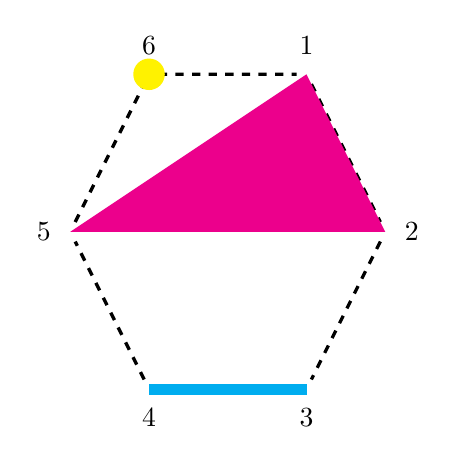
\begin{tikzpicture}[scale=1]
            \node [label = above : {$1$}] (1)
                at (4,5) {};
            \node [label = right : {$2$}] (2)
                at (5,3) {};
            \node [label = below : {$3$}] (3)
                at (4,1) {};
            \node [label = below : {$4$}] (4)
                at (2,1) {};
            \node [label = left : {$5$}]  (5)
                at (1,3) {};
            \node [label = above : {$6$}] (6)
                at (2,5) {};
            \draw [dashed][very thick]
            (1) -- (2) -- (3) -- (4)
                -- (5) -- (6) -- (1);
            \fill [color = magenta] (4,5) -- (5,3)
                -- (1,3) -- cycle;
            \draw [color = cyan][line width = 4pt] 
                (4,1) -- (2,1);
            \fill [color=yellow] (2,5) circle (0.2);
          \end{tikzpicture}
    \end{center}
\end{example}

Thus non-crossing meaning the hulls are \emph{disjoint}.\\

\subsection{The non-crossing partitions poset}

\begin{definition}[$\succ$]
    We say that $P$ covers $Q$, written $P \succ Q$,
    if $\exists B_i, B_j \in P$ such that
    $Q = P - \{B_i, B_j\} \cup \{B_i \cup B_j\}$    
\end{definition}

\begin{example}
    $\{\{1, 6\}, \{2, 3\}, \{4, 5\}\} \succ
    \{\{1, 2, 3, 6\}, \{4, 5\}\}$\\
    \begin{itemize*}
        \item $B_i = \{1, 6\}$\\
        \item $B_j = \{2, 3\}$\\
    \end{itemize*}
\end{example}

\begin{prop}
    This covering relation defines the \emph{poset}
    of $\mathcal{NC}_n$.
    We denote by $\mathcal{NCC}_n$ the set of
    \emph{maximal chains} in the poset of $\mathcal{NC}_n$.\\
    $$\mathcal{NCC} = \bigcup_{n > 0}{\mathcal{NCC}_n}$$
\end{prop}

\begin{rem}
    The bottom element of this poset is $\{\{1, \ldots, n\}\}$,
    and the top element is $\{\{1\}, \ldots, \{n\}\}$.
\end{rem}

\begin{theorem}
    Let $ncc_n$ be the cardinal of $\mathcal{NCC}_n$.
    We have $$ncc_n = n^{n - 2}$$.
\end{theorem}

\begin{example}[The poset of $\mathcal{NC}_4$]
    ~\\
    To shorten labels, we represent $\{\{1\}, \{2, 3\},
    \{4\}\}$ by $1|23|4$. \\

    \begin{center}
        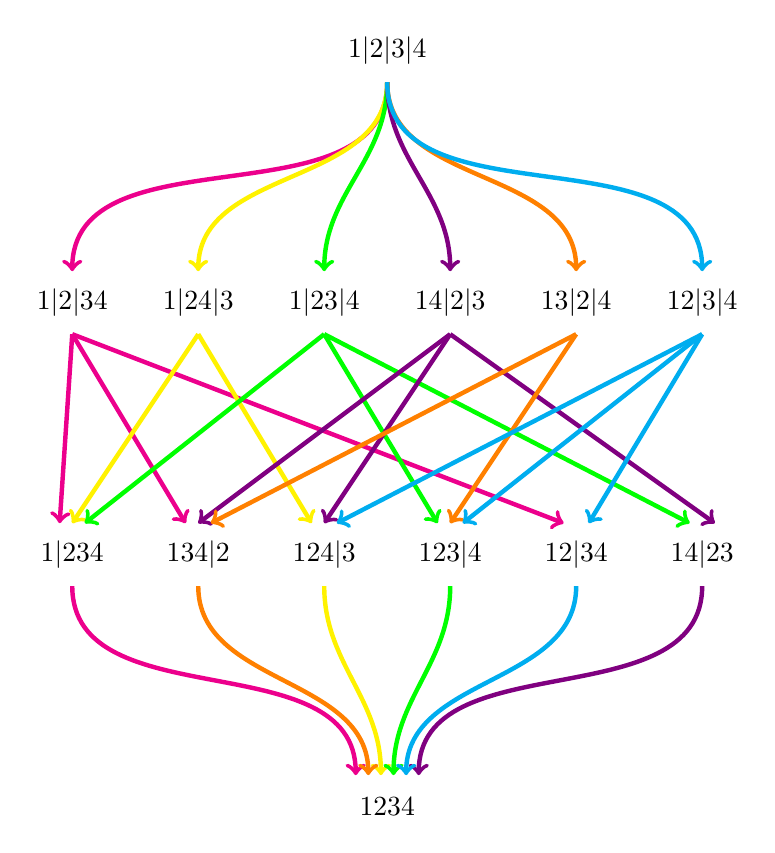
\begin{tikzpicture}[scale = 0.8]
            \node (0)  at (0,0)  {$1234$};
            \node (1)  at (-5,4) {$1|234$};
            \node (2)  at (-3,4) {$134|2$};
            \node (3)  at (-1,4) {$124|3$};
            \node (4)  at (1,4)  {$123|4$};
            \node (5)  at (3,4)  {$12|34$};
            \node (6)  at (5,4)  {$14|23$};
            \node (7)  at (-5,8) {$1|2|34$};
            \node (8)  at (-3,8) {$1|24|3$};
            \node (9)  at (-1,8) {$1|23|4$};
            \node (10) at (1,8)  {$14|2|3$};
            \node (11) at (3,8)  {$13|2|4$};
            \node (12) at (5,8)  {$12|3|4$};
            \node (13) at (0,12) {$1|2|3|4$};
        
            \draw [->][out=-90,in=90, ultra thick] 
                [color=magenta](0,11.5) to (-5,8.5);
            \draw [->][color=magenta, ultra thick]
                (-5,7.5) to (-5.2,4.5);
            \draw [->][color=magenta, ultra thick]
                (-5,7.5) to (-3.2,4.5); 
            \draw [->][color=magenta, ultra thick]
                (-5,7.5) to (2.8,4.5);
            \draw [->][out=-90,in=90, ultra thick] 
                [color=magenta](-5,3.5) to (-0.5,0.5);
        
            \draw [->][out=-90,in=90, ultra thick]
                [color=yellow] (0,11.5) to (-3,8.5);
            \draw [->][color=yellow, ultra thick]
                (-3,7.5) to (-5,4.5);
            \draw [->][color=yellow, ultra thick]
                (-3,7.5) to (-1.2,4.5);
            \draw [->][out=-90,in=90, ultra thick] 
                [color=yellow](-1,3.5) to (-0.1,0.5);
            
            \draw [->][out=-90,in=90, ultra thick]
                [color=green](0,11.5) to (-1,8.5);
            \draw [->][color=green, ultra thick]
                (-1,7.5) to (-4.8,4.5);
            \draw [->][color=green, ultra thick]
                (-1,7.5) to (0.8,4.5);
            \draw [->][color=green, ultra thick]
                (-1,7.5) to (4.8,4.5);
            \draw [->][out=-90,in=90, ultra thick] 
                [color=green](1,3.5) to (0.1,0.5);
        
            \draw [->][out=-90,in=90, ultra thick]
                [color=violet](0,11.5) to (1,8.5);
            \draw [->][color=violet, ultra thick]
                (1,7.5) to (-3,4.5);
            \draw [->][color=violet, ultra thick]
                (1,7.5) to (-1,4.5);
            \draw [->][color=violet, ultra thick]
                (1,7.5) to (5.2,4.5);
            \draw [->][out=-90,in=90, ultra thick] 
                [color=violet](5,3.5) to (0.5,0.5);
        
            \draw [->][out=-90,in=90, ultra thick]
                [color=orange](0,11.5) to (3,8.5);
            \draw [->][color=orange, ultra thick]
                (3,7.5) to (-2.8,4.5);
            \draw [->][color=orange, ultra thick]
                (3,7.5) to (1,4.5);
            \draw [->][out=-90,in=90, ultra thick] 
                [color=orange](-3,3.5) to (-0.3,0.5);
        
            \draw [->][out=-90,in=90, ultra thick]
                [color=cyan](0,11.5) to (5,8.5);
            \draw [->][color=cyan, ultra thick]
                (5,7.5) to (-0.8,4.5);
            \draw [->][color=cyan, ultra thick]
                (5,7.5) to (1.2,4.5);
            \draw [->][color=cyan, ultra thick]
                (5,7.5) to (3.2,4.5);
            \draw [->][out=-90,in=90, ultra thick] 
                [color=cyan](3,3.5) to (0.3,0.5);
        
        \end{tikzpicture}
        ~\\
        ~\\
        There are $4^2 = 16$ different maximal chains,
        and $\frac {1}{5} \binom{8}{4} = \frac{70}{5} = 14$
        elements in this poset.
    \end{center}
\end{example}



\subsection{Kreweras complement}

\begin{definition}[Associated Permutation]
    The \emph{permutation} $\sigma$ associated to a non-crossing
    partition has a cycle $(b_1, \ldots, b_k)$ for each block
    $B = \{b_1, \ldots, b_k\}$ of the partition.
\end{definition}

\begin{example}
    The permutation associated to $\{\{1, 2, 5\}, \{3, 4\}, \{6\}\}$
    is $(1\ 2\ 5)\ (3\ 4)\ (6) = 254316$.
\end{example}

\begin{definition}[Kreweras Complement]
    The \emph{Kreweras complement} $K (P)$ of a non-crossing
    partition $P$ is defined as follows :\\
    \begin{itemize*}
        \item Let $\sigma$ be the permutation associated to $P$\\
        \item Let $\pi$ be the permutation $(n\ n-1\ n-2\
        \ldots\ 3\ 2\ 1) = n123 \ldots n-1$\\
        \item $K (P)$ is the \emph{non-crossing partition}
        associated to $\pi \sigma$.\\
    \end{itemize*}
\end{definition}

\begin{example}[$P = \{\{1, 2, 5\}, \{3, 4\}, \{6\}\}$]
    ~\\
    \begin{itemize*}
        \item $\sigma = (1\ 2\ 5)\ (3\ 4)\ (6) = 254316$\\
        \item $\pi = (6\ 5\ 4\ 3\ 2\ 1) = 612345$\\
        \item $\pi \sigma = 143265 = (1)\ (2\ 4)\ (3)\ (5\ 6)$\\
        \item $K(P) = \{\{1\},\{2, 4\}, \{3\}, \{5, 6\}\}$\\
    \end{itemize*}
\end{example}

\begin{prop}[Kreweras minimums]
        Let $P = \{B_1, \ldots, B_k\}$ be a non-crossing partition.
        Let $K (P) = \{B'_1, \ldots, B'_l\}$ be its Kreweras complement.
        Then $$\bigcup_{1 \leq i \leq l}{min (B'_i)} =
        B_1 \cup \bigcup_{1 < j \leq k}{B_i - {max (B_i)}}$$\\
\end{prop}

\begin{example}[$P = \{\{1, 2, 5\}, \{3, 4\}, \{6\}\}$]
    ~\\
    \begin{itemize}
        \item $K (P) = \{\{1\},\{2, 4\}, \{3\}, \{5, 6\}\}$
        \item $\bigcup{min (B'_i)} = \{1, 2, 3, 5\}$
        \item $B_1\ \cup\ \bigcup{B_i - {max (B_i)}}
        = \{1, 2, 5\} \cup \{3, 4\} - \{4\} \cup \{6\} - \{6\}
        = \{1, 2, 5\} \cup \{3\} \cup \emptyset = \{1, 2, 3, 5\}$\\
    \end{itemize}
\end{example}

\begin{notation}
    $B_{[i]} = $ block containing $i$.
\end{notation}

\begin{prop}[Kreweras block sizes]
    Let $P = \{B_1, \ldots, B_k\}$ be a non-crossing partition.
    Let $K (P) = \{B'_1, \ldots, B'_l\}$ be its Kreweras complement.
    Then the size of the block $B'_i$ is defined as follows :
    \begin{itemize}
        \item Let $m_i$ be the the $i^{th}$ minimum of $K (P)$
        \item Define a \emph{transition} $\phi (e)$ as 
            \subitem Let $j = e + 1$ (or $1$ if $e = n$)
            \subitem $\phi(e) = max (B_{[j]})$
        \item The size of $B'_i$ is $k_{min}$ such that
        $k_{min} = min \{k > 0\ |\ \phi^k (m_i) \in B_{[m_i]}\}$.\\
    \end{itemize}
\end{prop}

\begin{example}[$P = \{\{1, 2, 5\}, \{3, 4\}, \{6\}\}$]
    ~\\
    \begin{itemize}
        \item $mins = \{1, 2, 3, 5\}$
        \item $m_1 = 1$
            \subitem $B_{[1]} = B_1$
            \subitem $max (B_{[2]} = max (B_1) = 5$
            \subitem The size for $m_1$ is $1$.
        \item $m_2$
            \subitem $B_{[2]} = B_1$
            \subitem $max (B_{[3]}) = max (B_2) = 4$
            \subitem $max (B_{[5]}) = max (B_1) = 5$
            \subitem The size for $m_2$ is $2$.
        \item $m_3 = 3$
            \subitem $B_{[3]} = B_2$
            \subitem $max (B_{[4]}) = max (B_2) = 4$
            \subitem The size for $m_3$ is $1$.
        \item $m_4 = 5$
            \subitem $B_{[5]} = B_1$
            \subitem $max (B_{[6]}) = max (B_3) = 6$
            \subitem $max (B_{[1]}) = max (B_1) = 5$
            \subitem The size for $m_4$ is $2$.
    \end{itemize}
\end{example}

\subsection{Action of $\mathfrak{S}_n$ on $\mathcal{NC}_n$}

\begin{definition}[Action of $\mathfrak{S}_n$]
    The action of $\mathfrak{S}_n$ on a non-crossing partition
    $P = \{B_1, \ldots, B_l\} \in \mathcal{NC}_n$ is defined by :\\
    \begin{itemize*}
        \item For each block $B_i = \{b_1, \ldots, b_k\}$ :
        $\sigma(Bi) =\{\sigma (b_1), \ldots, \sigma (b_k)\}$ \\
        \item We denote $\rho = \sigma(P) =
            \{\sigma (B_1), \ldots, \sigma (B_l)\}$
    \end{itemize*}
\end{definition}

\begin{example}[$\sigma = 415362$]
    ~\\
    $\sigma (\{\{1, 6\}, \{2, 3, 5\}, \{4\}\}) = 
        \{\{1, 5, 6\}, \{2, 4\}, \{3\}\}$
\end{example}

\begin{rem}
    Note that $\sigma (P)$ is \emph{not} necessarily
    non-crossing.
\end{rem}

\begin{definition}[Rotation]
    We define the \emph{rotation operator} $rot$ of
    $P \in \mathcal{NC}_n$ as $rot (P) = 
    (1\ 2\ 3\  \ldots \ n)(P) = 23 \ldots n1 (P)$.\\
    Conversely, we define $rot^{-1}$ of $P$ as
    $rot^{-1}(P) = (n\ n-1\ \ldots 3\ 2\ 1)(P) = 
    n12 \ldots n-1 (P)$.
\end{definition}

\begin{rem}
    $K (K (P)) = rot^{-1} (P)$.
\end{rem}

\begin{example}[$P = \{\{1, 6\}, \{2, 3, 5\}, \{4\}\}$]
    ~\\
    \begin{itemize}
        \item $rot (P) = \{\{1, 2\}, \{3, 4, 6\}, \{5\}\}$
        \item $rot^{-1}(P) = \{\{1, 2, 4\}, \{3\}, \{5, 6\}\}$
    \end{itemize}
    
\end{example}

\section{Non-crossing 2-partitions}

\begin{definition}[Non-crossing 2-partition]
    A \emph{non-crossing 2-partition} of a set $E$ is a pair $(P, \sigma)$
    where :\\
    \begin{itemize*}
        \item $P$ is a non-crossing partition of $E$\\
        \item $\sigma$ is a permutation of the elements of $E$\\
        \item For each \emph{sorted} block
            $B_i = \{b_1, \ldots, b_k\} \in P$, we have
            $\sigma (b_i) < \ldots < \sigma (b_k)$\\\\
    \end{itemize*}
    We denote by $\mathcal{NC}^2_n$ the set of non-crossing
    2-partitions of $[n]$.
    $$\mathcal{NC}^2 = \bigcup_{n > 0}{\mathcal{NC}^2_n}$$.
\end{definition}

\begin{example}[$\mathcal{NC}^2_6$]
    \begin{itemize*}
            \subitem $P = \{\{1, 6\}, \{2, 3, 5\}, \{4\}\}$
            \subitem $\sigma = 413265$ \\
            \subitem $\hspace{36mm} \rho = \{\{1, 3, 6\}, \{2\}, \{4, 5\}\}$
    \end{itemize*}    
\end{example}

\begin{theorem}
    Let $nc^2_n$ be the cardinal of $\mathcal{NC}^2_n$.
    We have $$nc^2_n = (n + 1)^{n-1}$$
\end{theorem}

\begin{example}[$n = 1, 2, 3$]
    ~\\
    \begin{itemize}
            \item $n = 1$ \  $:$ \  $nc^2_1 = 1$
            \subitem $\{\{1\}\}$ \hspace{1cm} $1$
                \hspace{1cm} $\rho = P$
            \item $n = 2$ \  $:$ \  $nc^2_2 = 3$
            \subitem $\{\{1\}, \{2\}\}$ \hspace{1cm} $12$
                \hspace{1cm} $\rho = P$
            \subitem $\{\{1\}, \{2\}\}$ \hspace{1cm} $21$
                \hspace{1cm} $\rho = P$
            \subitem $\{\{1, 2\}\}$ \hspace{14mm} $12$
                \hspace{1cm} $\rho = P$
            \item $n = 3$ \  $:$ \  $nc^2_3 = 16$
            \subitem $\{\{1\}, \{2\}, \{3\}\}$ \hspace{1cm}
                $123$ \hspace{1cm} $\rho = P$
            \subitem $\{\{1\}, \{2\}, \{3\}\}$ \hspace{1cm}
                $132$ \hspace{1cm} $\rho = P$
            \subitem $\{\{1\}, \{2\}, \{3\}\}$ \hspace{1cm}
                $213$ \hspace{1cm} $\rho = P$
            \subitem $\{\{1\}, \{2\}, \{3\}\}$ \hspace{1cm}
                $231$ \hspace{1cm} $\rho = P$
            \subitem $\{\{1\}, \{2\}, \{3\}\}$ \hspace{1cm}
                $312$ \hspace{1cm} $\rho = P$
            \subitem $\{\{1\}, \{2\}, \{3\}\}$ \hspace{1cm}
                $321$ \hspace{1cm} $\rho = P$       
            \subitem $\{\{1, 2\}, \{3\}\}$ \hspace{14mm}
                $123$ \hspace{1cm} $\rho = P$
            \subitem $\{\{1, 2\}, \{3\}\}$ \hspace{14mm}
                $132$ \hspace{1cm} $\rho = \{\{1, 3\}, \{2\}\}$
            \subitem $\{\{1, 2\}, \{3\}\}$ \hspace{14mm}
                $231$ \hspace{1cm} $\rho = \{\{1\}, \{2, 3\}\}$
            \subitem $\{\{1\}, \{2, 3\}\}$ \hspace{14mm}
                $123$ \hspace{1cm} $\rho = P$
            \subitem $\{\{1\}, \{2, 3\}\}$ \hspace{14mm}
                $213$ \hspace{1cm} $\rho = \{\{1, 3\}, \{2\}\}$
            \subitem $\{\{1\}, \{2, 3\}\}$ \hspace{14mm}
                $312$ \hspace{1cm} $\rho = \{\{1, 2\}, \{3\}\}$
            \subitem $\{\{1, 3\}, \{2\}\}$ \hspace{14mm}
                $123$ \hspace{1cm} $\rho = P$
            \subitem $\{\{1, 3\}, \{2\}\}$ \hspace{14mm}
                $132$ \hspace{1cm} $\rho = \{\{1, 2\}, \{3\}\}$
            \subitem $\{\{1, 3\}, \{2\}\}$ \hspace{14mm}
                $213$ \hspace{1cm} $\rho = \{\{1\}, \{2, 3\}\}$  
            \subitem $\{\{1, 2, 3\}\}$ \hspace{18mm}
                $123$ \hspace{1cm} $\rho = P$\\
    \end{itemize}
\end{example}

\begin{prop}
    This means we can create a \emph{bijection} between
    $\mathcal{PF}_n$ and $\mathcal{NC}^2_n$.
\end{prop}

\begin{proof}
    ~\\
\begin{itemize}
    \item $\mathcal{PF}_n \to \mathcal{NC}^2_n$ :
    Let $f = (a_1, \ldots, a_n) \in \mathcal{PF}_n$
    be our parking function.
    For $i \in \{1, \ldots, n\}$, we define :
        \subitem $l_i$ : the number of occurences of $i$ in $f$. 
        \subitem $im_i$ : $\{j\ |\ a_j = i\}$\\
    The corresponding non-crossing partition will
    have the following constraints :
        \subitem For each $i \in \{1, \ldots, n\}$, if $l_i > 0$,
        then there is a block $B_{[i]}$ of length
        \subitem $l_i$ with minimum element $i$.
        \subitem $\sigma (B_{[i]}) = im_i$\\
    There is a unique set partition
    $\displaystyle P = \bigcup_{i}{B}_{[i]}$ of $[n]$
    and a unique permutation $\sigma$ respecting these
    conditions such that $(P, \sigma) \in \mathcal{NC}^2_n$.
    \item $\mathcal{NC}^2_n \to \mathcal{PF}_n$ :
    Let $(P, \sigma)$ with $P = \{B_1, \ldots, B_l\}$ be our
    non-crossing 2-partition.
    For each block $B_i = \{b_1, \ldots, b_k\} \in P$ :
    \subitem $m_i = min (B_i) = b_1$
    \subitem $pos_i = \sigma (B_i)$
    \subitem For each $j \in pos_i$, we define $a_j = m_i$\\
    The corresponding parking function is $(a_1, \ldots, a_n)$.
\end{itemize}
\end{proof}

\begin{example}[$n = 8$]
    \begin{align*}
        &P = \{\{1, 2, 5\}, \{3, 4\}, \{6, 8\}, \{7\}\}\\
        &\sigma = 36187245\\
        &f = (3, 6, 1, 7, 6, 1, 1, 3)\\
    \end{align*}
\end{example}

\subsection{The non-crossing 2-partitions poset}

\begin{definition}[$\succ^2$]
    We say that $(P, \sigma)$ covers $(Q, \tau)$, written
    ($P, \sigma) \succ^2 (Q, \tau)$,
    if $\exists B_i, B_j \in P$ such that\\
    \begin{itemize*}
        \item $Q = P - \{B_i, B_j\} \cup \{B_i \cup B_j\}$\\
        \item $l \neq i, j \and b \in B_l \rightarrow
            \tau (b) = \sigma (b)$\\
        \item Let $B_i \cup B_j = \{b_1, \ldots, b_k\}$ :\\
            \subitem $\tau (B_i \cup B_j) = \sigma (B_i \cup B_j)$\\
            \subitem $\tau (b_1) < \ldots < \tau (b_k)$
    \end{itemize*}    
\end{definition}

\begin{example}
    ~\\
    \begin{itemize*}
        \item $P = \{\{1, 6\}, \{2, 3\}, \{4\}, \{5\}\}$\\
        \item $\sigma = 236154$\\
        \item $Q = \{\{1, 6\}, \{2, 3, 5\}, \{4\}\}$\\
        \item $\tau = 235164$\\
        \item $(P, \sigma) \succ^2 (Q, \tau)$\\
        \item $(P, \sigma) \not \succ^2 (Q, \sigma)$,
        because  $\sigma (\{2, 3, 5\}) = \{3, 6, 5\}$ is
        \emph{not} ordemagenta. 
    \end{itemize*}
\end{example}

\begin{prop}
    This covering relation defines the \emph{poset} of
    $\mathcal{NC}^2_n$.
\end{prop}

\begin{rem}
    The bottom element of this poset is 
    $(\{\{1, \ldots, n\}\}, 12 \ldots n)$, and the top
    elements are $\{(\{\{1\}, \ldots, \{n\}\}, \sigma)\ 
    |\ \sigma \in \mathfrak{S}_n\}$.
\end{rem}

\begin{example}[The poset of $\mathcal{NC}^2_3$]
    ~\\
    To shorten labels, we represent
    $(\{\{1, 3\}, \{2\}\}, 213)$ by \\
    \begin{center}
        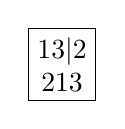
\begin{tikzpicture}
            \node (0) at (0,0) [align = center]
            [rectangle, draw]{$13|2$\\$213$};
        \end{tikzpicture}
    \end{center}

    \begin{center}
        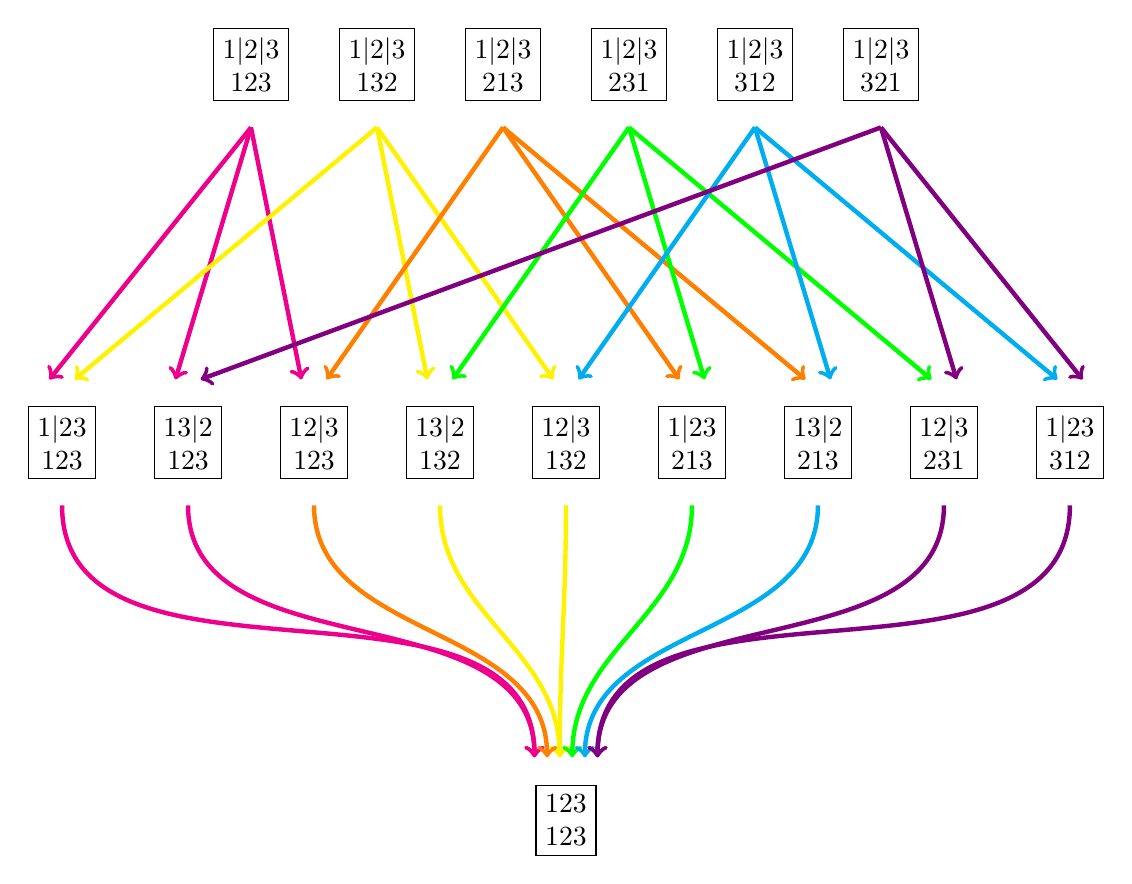
\begin{tikzpicture}[scale = 0.8]
            \node (0)  at (0,0) [align = center]
            [rectangle, draw]
                {$123$\\$123$};
            \node (1)  at (-8,6)[align = center]
            [rectangle, draw]
                {$1|23$\\$123$};
            \node (2)  at (-6,6) [align = center]
            [rectangle, draw]
                {$13|2$\\$123$};
            \node (3)  at (-4,6) [align = center]
            [rectangle, draw]
                {$12|3$\\$123$};
            \node (4)  at (-2,6) [align = center]
            [rectangle, draw]
                {$13|2$\\$132$};
            \node (5)  at (0,6) [align = center]
            [rectangle, draw]
                {$12|3$\\$132$};
            \node (6)  at (2,6) [align = center]
            [rectangle, draw]
                {$1|23$\\$213$};
            \node (7)  at (4,6) [align = center]
            [rectangle, draw]
                {$13|2$\\$213$};
            \node (8)  at (6,6) [align = center]
            [rectangle, draw]
                {$12|3$\\$231$};
            \node (9)  at (8,6) [align = center]
            [rectangle, draw]
                {$1|23$\\$312$};
            \node (10) at (-5,12) [align = center]
            [rectangle, draw]
                {$1|2|3$\\$123$};
            \node (11) at (-3,12) [align = center]
            [rectangle, draw]
                {$1|2|3$\\$132$};
            \node (12) at (-1,12) [align = center]
            [rectangle, draw]
                {$1|2|3$\\$213$};
            \node (13) at (1,12) [align = center]
            [rectangle, draw]
                {$1|2|3$\\$231$};
            \node (14) at (3,12) [align = center]
            [rectangle, draw]
                {$1|2|3$\\$312$};
            \node (15) at (5,12) [align = center]
            [rectangle, draw]
                {$1|2|3$\\$321$};
        
            \draw [->][color=magenta, ultra thick]
                (-5,11) to (-8.2,7);
            \draw [->][color=magenta, ultra thick]
                (-5,11) to (-6.2, 7); 
            \draw [->][color=magenta, ultra thick]
                (-5,11) to (-4.2,7);
            \draw [->][out=-90,in=90, ultra thick] 
                [color=magenta](-8,5) to (-0.5,1);
            \draw [->][out=-90,in=90, ultra thick] 
                [color=magenta](-6,5) to (-0.5,1);
        
            \draw [->][color=yellow, ultra thick]
                (-3,11) to (-7.8,7);
            \draw [->][color=yellow, ultra thick]
                (-3,11) to (-2.2,7);
            \draw [->][color=yellow, ultra thick]
                (-3,11) to (-0.2, 7);
            \draw [->][out=-90,in=90, ultra thick] 
                [color=yellow](-2,5) to (-0.1,1);
            \draw [->][out=-90,in=90, ultra thick] 
                [color=yellow](0,5) to (-0.1,1);
            
            \draw [->][color=orange, ultra thick]
                (-1,11) to (1.8,7);
            \draw [->][color=orange, ultra thick]
                (-1,11) to (3.8,7);
            \draw [->][color=orange, ultra thick]
                (-1,11) to (-3.8,7);
            \draw [->][out=-90,in=90, ultra thick] 
                [color=orange](-4,5) to (-0.3,1);
        
            \draw [->][color=green, ultra thick]
                (1,11) to (2.2,7);
            \draw [->][color=green, ultra thick]
                (1,11) to (-1.8,7);
            \draw [->][color=green, ultra thick]
                (1,11) to (5.8,7);
            \draw [->][out=-90,in=90, ultra thick] 
                [color=green](2,5) to (0.1,1);
        
            \draw [->][color=cyan, ultra thick]
                (3,11) to (7.8,7);
            \draw [->][color=cyan, ultra thick]
                (3,11) to (4.2,7);
            \draw [->][color=cyan, ultra thick]
                (3,11) to (0.2,7);
            \draw [->][out=-90,in=90, ultra thick] 
                [color=cyan](4,5) to (0.3,1);
        
            \draw [->][color=violet, ultra thick]
                (5,11) to (8.2,7);
            \draw [->][color=violet, ultra thick]
                (5,11) to (-5.8,7);
            \draw [->][color=violet, ultra thick]
                (5,11) to (6.2,7);
            \draw [->][out=-90,in=90, ultra thick] 
                [color=violet](6,5) to (0.5,1);
            \draw [->][out=-90,in=90, ultra thick] 
                [color=violet](8,5) to (0.5,1);
            
        \end{tikzpicture}
        ~\\
        There are $4^2 = 16$ elements in this poset.
    \end{center}
\end{example}

\subsection{The parking functions poset}

\begin{definition}[Rank]
    Given $f = (a_1, \ldots, a_n) \in \mathcal{PF}_n$, let
    $$b_i =
    \begin{cases}
        1 \text{ if } \exists j\ |\ a_j = i\\
        0 \text{ otherwise}
    \end{cases} $$
    We define the \emph{rank} of $f$, noted $rk(f)$, as
    $$\sum_{1 \leq i \leq n}{b_i}$$
\end{definition}

\begin{example}
    \begin{align*}
        &rk((1, 5, 4, 2, 3, 3, 1)) = 5\\
        &rk((4, 7, 1, 1, 3, 2 ,2, 8)) = 6\\
    \end{align*}
\end{example}

\begin{definition}[$\succ_{pf}$]
    Since $\mathcal{PF}_n$ and $\mathcal{NC}^2_n$ are
    in bijection, we can define a \emph{covering relation}
    $\succ_{pf}$ for $\mathcal{PF}_n$ as follows :\\
    $f \in \mathcal{PF}_n \succ_{pf} g \in \mathcal{PF}_n$
    if and only if :    
    \begin{itemize}
        \item $(P,\sigma)$ is the non-crossing 2-partition
        associated to $f$
        \item $(Q, \tau)$ is the non-crossing 2-partition
        associated to $g$
        \item $(P, \sigma) \succ^2 (Q, \tau)$
    \end{itemize}
\end{definition}

\begin{example}
    ~\\
    \begin{itemize*}
        \item $P = \{\{1, 6\}, \{2, 3\}, \{4\}, \{5\}\}$\\
        \item $\sigma = 236154$\\
        \item $Q = \{\{1, 6\}, \{2, 3, 5\}, \{4\}\}$\\
        \item $\tau = 235164$\\
        \item $f = (4, 1, 2, 1, 5, 2) \succ_{pf}
            g = (4, 1, 2, 1, 2, 2)$\\
    \end{itemize*}
\end{example}

\begin{rem}
    If $f \succ_{pf} g$, then $rk(f) = rk(g) + 1$, and
    there exists $i$ and $j$ such that :
    \begin{itemize}
        \item $i < j$
        \item There is at least $1$ occurence of $i$ in $f$
        \item There is at least $1$ occurence of $j$ in $f$
        $$b_k =
            \begin{cases}
                i \text{ if } a_k = j\\
                a_k \text{ otherwise}\\
            \end{cases}$$
    \end{itemize}
\end{rem}

\begin{prop}
    This covering relation defines the \emph{poset}
    of $\mathcal{PF}_n$.
\end{prop}

\begin{rem}
    The bottom element of this poset is
    $(\underbrace{1, \ldots, 1}_{n})$,
    and the top elements are the \emph{permutations} of
    $\{1, \ldots, n\}$.
\end{rem}

\begin{example}[The poset of $\mathcal{PF}_3$]
    ~\\
    \begin{center}
        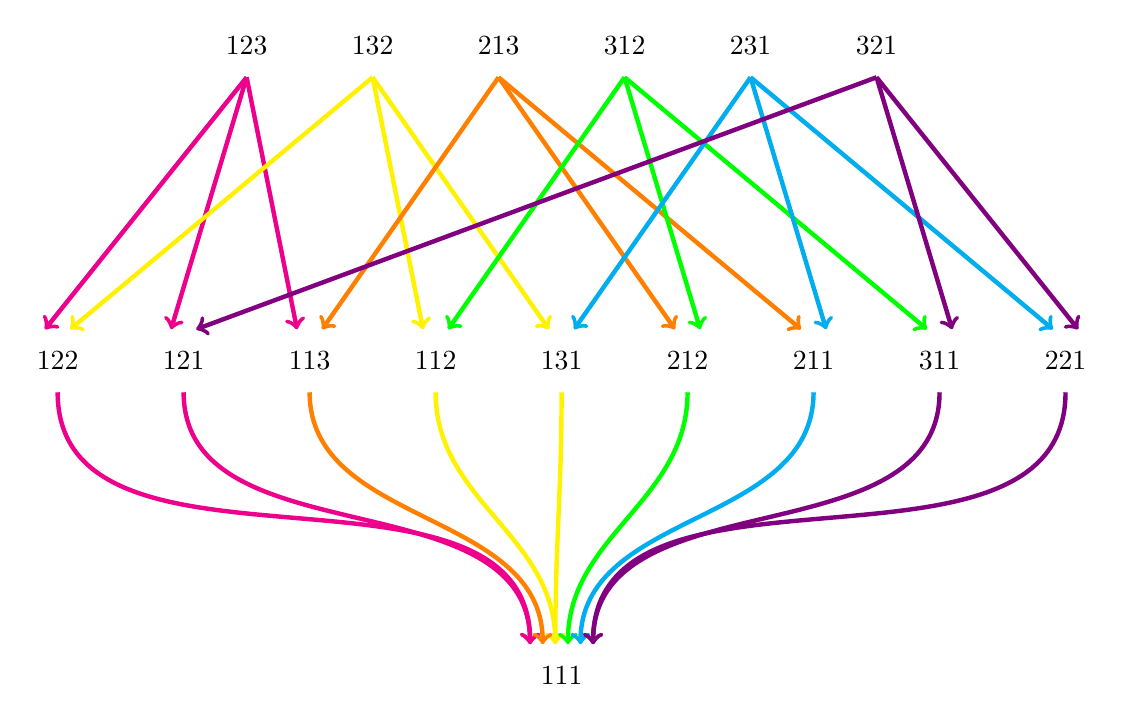
\begin{tikzpicture}[scale = 0.8]
            \node (0)  at (0,0)   {$111$};
            \node (1)  at (-8,5)  {$122$};
            \node (2)  at (-6,5)  {$121$};
            \node (3)  at (-4,5)  {$113$};
            \node (4)  at (-2,5)  {$112$};
            \node (5)  at (0,5)   {$131$};
            \node (6)  at (2,5)   {$212$};
            \node (7)  at (4,5)   {$211$};
            \node (8)  at (6,5)   {$311$};
            \node (9)  at (8,5)   {$221$};
            \node (10) at (-5,10) {$123$};
            \node (11) at (-3,10) {$132$};
            \node (12) at (-1,10) {$213$};
            \node (13) at (1,10)  {$312$};
            \node (14) at (3,10)  {$231$};
            \node (15) at (5,10)  {$321$};
        
            \draw [->][color=magenta, ultra thick]
                (-5,9.5) to (-8.2,5.5);
            \draw [->][color=magenta, ultra thick]
                (-5,9.5) to (-6.2,5.5); 
            \draw [->][color=magenta, ultra thick]
                (-5,9.5) to (-4.2,5.5);
            \draw [->][out=-90,in=90, ultra thick] 
                [color=magenta](-8,4.5) to (-0.5,0.5);
            \draw [->][out=-90,in=90, ultra thick] 
                [color=magenta](-6,4.5) to (-0.5,0.5);
        
            \draw [->][color=yellow, ultra thick]
                (-3,9.5) to (-7.8,5.5);
            \draw [->][color=yellow, ultra thick]
                (-3,9.5) to (-2.2,5.5);
            \draw [->][color=yellow, ultra thick]
                (-3,9.5) to (-0.2,5.5);
            \draw [->][out=-90,in=90, ultra thick] 
                [color=yellow](-2,4.5) to (-0.1,0.5);
            \draw [->][out=-90,in=90, ultra thick] 
                [color=yellow](0,4.5) to (-0.1,0.5);
            
            \draw [->][color=orange, ultra thick]
                (-1,9.5) to (1.8,5.5);
            \draw [->][color=orange, ultra thick]
                (-1,9.5) to (3.8,5.5);
            \draw [->][color=orange, ultra thick]
                (-1,9.5) to (-3.8,5.5);
            \draw [->][out=-90,in=90, ultra thick] 
                [color=orange](-4,4.5) to (-0.3,0.5);
        
            \draw [->][color=green, ultra thick]
                (1,9.5) to (2.2,5.5);
            \draw [->][color=green, ultra thick]
                (1,9.5) to (-1.8,5.5);
            \draw [->][color=green, ultra thick]
                (1,9.5) to (5.8,5.5);
            \draw [->][out=-90,in=90, ultra thick] 
                [color=green](2,4.5) to (0.1,0.5);
        
            \draw [->][color=cyan, ultra thick]
                (3,9.5) to (7.8,5.5);
            \draw [->][color=cyan, ultra thick]
                (3,9.5) to (4.2,5.5);
            \draw [->][color=cyan, ultra thick]
                (3,9.5) to (0.2,5.5);
            \draw [->][out=-90,in=90, ultra thick] 
                [color=cyan](4,4.5) to (0.3,0.5);
        
            \draw [->][color=violet, ultra thick]
                (5,9.5) to (8.2,5.5);
            \draw [->][color=violet, ultra thick]
                (5,9.5) to (-5.8,5.5);
            \draw [->][color=violet, ultra thick]
                (5,9.5) to (6.2,5.5);
            \draw [->][out=-90,in=90, ultra thick] 
                [color=violet](6,4.5) to (0.5,0.5);
            \draw [->][out=-90,in=90, ultra thick] 
                [color=violet](8,4.5) to (0.5,0.5);
            
        \end{tikzpicture}
    \end{center}
\end{example}

\chapter{The rational case}

For the whole chapter, we will consider 2 \emph{coprime}
integers $a$ and $b$ (meaning $a$ and $b$ have $1$ as their
greatest common divisor).

\section{Rational Parking Functions}

\begin{definition}[a, b - Parking Function]
    An \emph{a, b - parking function} is a sequence 
    $(a_1, a_2, \ldots, a_n)$ such that :\\
    \begin{itemize*}
        \item $n = a$\\
        \item its non-decreasing reordering 
        $(b_1, b_2, \ldots, b_n)$
        has $b_i \leqslant \frac{b}{a}(i-1) + 1$
        for all $i$.\\\\
    \end{itemize*}
    We denote by $\mathcal{PF}_{a,b}$ the set of 
    a, b - parking functions.
\end{definition}

\begin{example}
    ~\\
    \begin{itemize}
        \item Ex. 1 : $a > b$
            \subitem $a = 7$
            \subitem $b = 3$
            \subitem Limits of the non-decreasing
            reordering of any $f \in \mathcal{PF}_{7,3}$ :
            \subitem $[1,\ 1 \frac{3}{7},\ 1 \frac{6}{7},\ 
            2 \frac{2}{7},\ 2 \frac{5}{7},\ 3 \frac{1}{7},\ 
            3 \frac{4}{7}]$
            \subitem $f_1 = (2, 1, 1, 3, 2, 3, 1) \in
            \mathcal{PF}_{7,3}$
            \subitem $f_2 = (2, 1, 2, 3, 2, 3, 1) \notin
            \mathcal{PF}_{7,3}$, even though $f_2 \in
            \mathcal{PF}_7$
        \item Ex. 2 : $a < b$
            \subitem $a = 5$
            \subitem $b = 7$
            \subitem Limits of the non-decreasing            
            reordering of any $f \in \mathcal{PF}_{5,7}$ :
            \subitem $[1,\ 2 \frac{2}{5},\ 3 \frac{4}{5},\ 
            5 \frac{1}{5},\ 6 \frac{3}{5}]$
            \subitem $f_3 = (6, 3, 5, 1, 2) \in
            \mathcal{PF}_{5,7}$, even though $f_3 \notin
            \mathcal{PF}_5$
            \subitem $f_4 = (6, 3, 5, 1, 3) \notin
            \mathcal{PF}_{5,7}$\\
    \end{itemize}
\end{example}

\begin{theorem}
    Let $pf_{a,b}$ be the cardinal of $\mathcal{PF}_{a,b}$.
    We have $$pf_{a,b} = b^{a-1}$$
\end{theorem}

\begin{example}[$a = 3, b = 5$]
    ~\\
    \begin{itemize*}\\
        \item $pf_{a,b} = 25$
        \item Limits : $[1,\ 2 \frac{2}{3},\ 
            4 \frac{1}{3}]$\\\\
        \subitem $(1, 1, 1)$
        \subitem $(1, 1, 2)$
        \subitem $(1, 1, 3)$
        \subitem $(1, 1, 4)$
        \subitem $(1, 2, 1)$
        \subitem $(1, 2, 2)$
        \subitem $(1, 2, 3)$
        \subitem $(1, 2, 4)$
        \subitem $(1, 3, 1)$
        \subitem $(1, 3, 2)$
        \subitem $(1, 4, 1)$
        \subitem $(1, 4, 2)$
        \subitem $(2, 1, 1)$
        \subitem $(2, 1, 2)$
        \subitem $(2, 1, 3)$
        \subitem $(2, 1, 4)$
        \subitem $(2, 2, 1)$
        \subitem $(2, 3, 1)$
        \subitem $(2, 4, 1)$
        \subitem $(3, 1, 1)$
        \subitem $(3, 1, 2)$
        \subitem $(3, 2, 1)$
        \subitem $(4, 1, 1)$
        \subitem $(4, 1, 2)$
        \subitem $(4, 2, 1)$
    \end{itemize*}
\end{example}

\begin{rem}    
    $\mathcal{PF}_{n, n+1} = \mathcal{PF}_n$.
    In fact, we do have $b^{a-1} = (n+1)^{n-1}$.
\end{rem}

\subsection{Rational primitives parking functions}

\begin{definition}[Rational Primitive]
    A rational parking function $f$ is said
    \emph{primitive} if it is already in
    non-decreasing order.\\
    We denote by $\mathcal{PF'}_{a,b}$ the set of
    primitive a, b - parking functions.
\end{definition}

\begin{example}[$a = 4, b = 3$]
    Limits : $[1,\ 1 \frac{3}{4},\ 2 \frac{1}{2},\ 
    3 \frac{1}{4}]$
    \begin{align*}
        &f_1 = (1, 1, 2, 2) \in \mathcal{PF'}_{4,3}\\
        &f_2 = (1, 1, 2, 1) \notin \mathcal{PF'}_{4,3},
        \text{ even though } f_2 \in \mathcal{PF}_{4,3}.
    \end{align*}
\end{example}

\begin{theorem}
    Let $pf'_{a,b}$ be the cardinal of
    $\mathcal{PF'}_{a,b}$.
    We have $$\displaystyle pf'_{a,b} = 
    \frac{1}{a + b} \binom{a + b}{b}$$
    which is the \emph{rational Catalan number}
    $Cat(a,b)$.
\end{theorem}

\begin{example}[$a = 3, b = 5$]
    ~\\
    \begin{itemize*}
        \item $pf'_{a,b} = 7$
        \item Limits : $[1,\ 2 \frac{2}{3},\ 
            4 \frac{1}{3}]$\\\\
        \subitem $(1, 1, 1)$
        \subitem $(1, 1, 2)$
        \subitem $(1, 1, 3)$
        \subitem $(1, 1, 4)$
        \subitem $(1, 2, 2)$
        \subitem $(1, 2, 3)$
        \subitem $(1, 2, 4)$
    \end{itemize*}    
\end{example}

\begin{rem}
    $\mathcal{PF'}_{n,n+1} = \mathcal{PF'}_n$.
    In fact, we do have
    $$\frac{1}{n + n + 1} \binom{n + n + 1}{n + 1}
    = \frac{1}{2n + 1} \binom {2n + 1}{n + 1}
    = \frac{1}{2n + 1} \frac{(2n + 1)!}{n ! (n+1)!}$$
    $$= \frac{(2n)!}{n!(n+1)!}
    = \frac{1}{n+1} \frac{(2n)!}{n!n!}
    = \frac{1}{n+1} \binom{2n}{n}$$
\end{rem}

\section{Rational Non-crossing Partitions}

\begin{definition}[Mutually Non-crossing Partitions]
    2 partitions $P$ and $Q$ are said
    \emph{mutually non-crossing} if :\\
    \begin{itemize*}
        \item P is non-crossing\\
        \item Q is non-crossing\\
        \item For every block $B_i$ of $P$ and every
        block $B_j$ of $Q$, if $a,c \in B_i$ and
        $b, d \in B_j$, then we can \emph{not} have
        $a < b < c < d$, nor $a > b > c > d$.
    \end{itemize*}    
\end{definition}

\begin{definition}[a, b - Non-crossing Partition]
    An \emph{a, b - non-crossing partition} is
    a pair $(P,Q)$ such that :\\
    \begin{itemize*}
        \item $P, Q \in \mathcal{NC}_{b-1}$\\
        \item $P$ and $Q$ are mutually non-crossing.\\
        \item TODO : ADD THE CONDITION
    \end{itemize*}
\end{definition}

\begin{prop}
    This means we can create a \emph{bijection} between
    $\mathcal{PF'}_{a,b}$ and $\mathcal{NC}_{a,b}$.
\end{prop}

\begin{proof}
    ~\\
\begin{itemize}
    \item $\mathcal{NC}_{a,b} \to \mathcal{PF'}_{a,b}$ :
    
    \item $\mathcal{PF'}_{a,b} \to \mathcal{NC}_{a,b}$ :
\end{itemize}
\end{proof}

\chapter{Trees}

\end{document}